\section{Atoms, Nuclei, and Nucleons: A Brief History}

The notion of the atom, as well as the English word \textit{atom}
(from the Greek \textgreek{ἄτομος}--átomos--``uncuttable,''
itself composed of the etymological ``atoms''
\textgreek{ἀ}--a--``not''
and
\textgreek{τέμνω }--témnō--``I cut'') can be traced to the Presocratic Greek
philosophers Leucippus and Democritus~\cite{sep-atomism-ancient}.
They posited that the natural world consists of two fundamental
constituents--atoms and the void through which they move.


This theory was developed in response to the paradoxes of Zeno of
Elea, which appear to draw contradictory conclusions about ``plurality'' and
the possibility of motion, particularly if matter consists of infinitely divisible
constituent parts~\cite{sep-paradox-zeno}.
Zeno argued that traversing a finite distance required first traversing
infinitely many subdivisions of that distance--an apparent contradiction.
Democritus's model supposes smallest subdivision, rendering the finite distance
to be traversed a sum of finitely many parts.
Various configurations of varying kinds, shapes, and sizes of Democritus's
atoms were thought to be the origins of the sensible properties of macroscopic
matter.
These configurations collide with an animal's sensory organs and give rise to
sensory experience.


In the early 19th century, John Dalton formulated the first modern concept of
the atom as the fundamental building block of chemical compounds.
His theory held that every chemical element is composed of atoms of identical
type and that different elements are composed of atoms of different size and
weight.
Chemical compounds are composed of whole numbers of atoms and reactions
involving different compounds consist of a rearrangement of the constituent
atoms.


In 1828, while studying the plant \textit{Clarkia pulchella} immersed in water
under a microscope,
botanist Robert Brown~\cite{Brown_1828} noted the
the irregular motion of the plant's pollen on the surface of the water.
In 1905, Albert Einstein developed a model of this motion  arising from
collisions with individual water molecules~\cite{Einstein_1905}.
% if I include this do I have to start talking about the history of molecular theory? seems tedious
French physicist Jean Perrin's measurements of the sedimentation of small
particles in liquid confirmed Einstein's hypothesis, work for which he was
awarded the Nobel Prize in 1926.


Rutherford, Geiger, and Marsden carried out a series of experiments between
1908 and 1913 in which they fired a beam of alpha particles
at thin metal foils to study atomic-scale structure~\cite{Rutherford_1911}.
The distribution of scattered particles they observed suggested that the atom
is composed of a small, dense, positively charged nucleus surrounded by a cloud
of electrons.

In the century since, physicists have used other particle beams to study the
substructure of nuclei as well as the nucleons (i.e. protons and neutrons)
that compose nuclei.
The culmination of decades of such experiments is a theory called quantum
chromodynamics (QCD): the theory that quarks and gluons are the fundamental
building blocks that make up hadrons, a category of composite particles that
includes protons and neutrons.
QCD also describes the interactions between such particles--the
\textit{strong nuclear force}.


QCD is part of the ``Standard Model'' of particle physics, which holds that
everything in the universe is made up of a handful of basic building blocks
whose interactions are governed by a few fundamental forces.
These building blocks, collectively called fermions, belong to two groups of
particles--quarks and leptons.
The quarks are typically found confined inside hadrons, while leptons can move
about more freely.
The interactions between these particles are mediated by force-carrying
particles called bosons that carry discrete packages of energy and momentum
between fermions.

Each of the three fundamental forces has one or more bosons associated with it.
The strong nuclear force, as mentioned above, has the gluon.
The electromagnetic force (quantum electrodynamics or QED) has the photon.
The weak nuclear force, responsible for beta decay among other things, has the
positively and negatively charged $W$ bosons and the neutral $Z$ boson.
There are a number of theories that have tried to incorporate the fourth
fundamental force, gravity, in a way that is consistent with the Standard
Model.
Unfortunately, this pursuit has proven difficult and no such theory has been
proven correct.
Figure~\ref{fig:Standard_Model_of_Elementary_Particles} displays the full list
of fundamental particles in the Standard Model, along with some of their
properties.

\begin{figure}[!h]
    \centering
    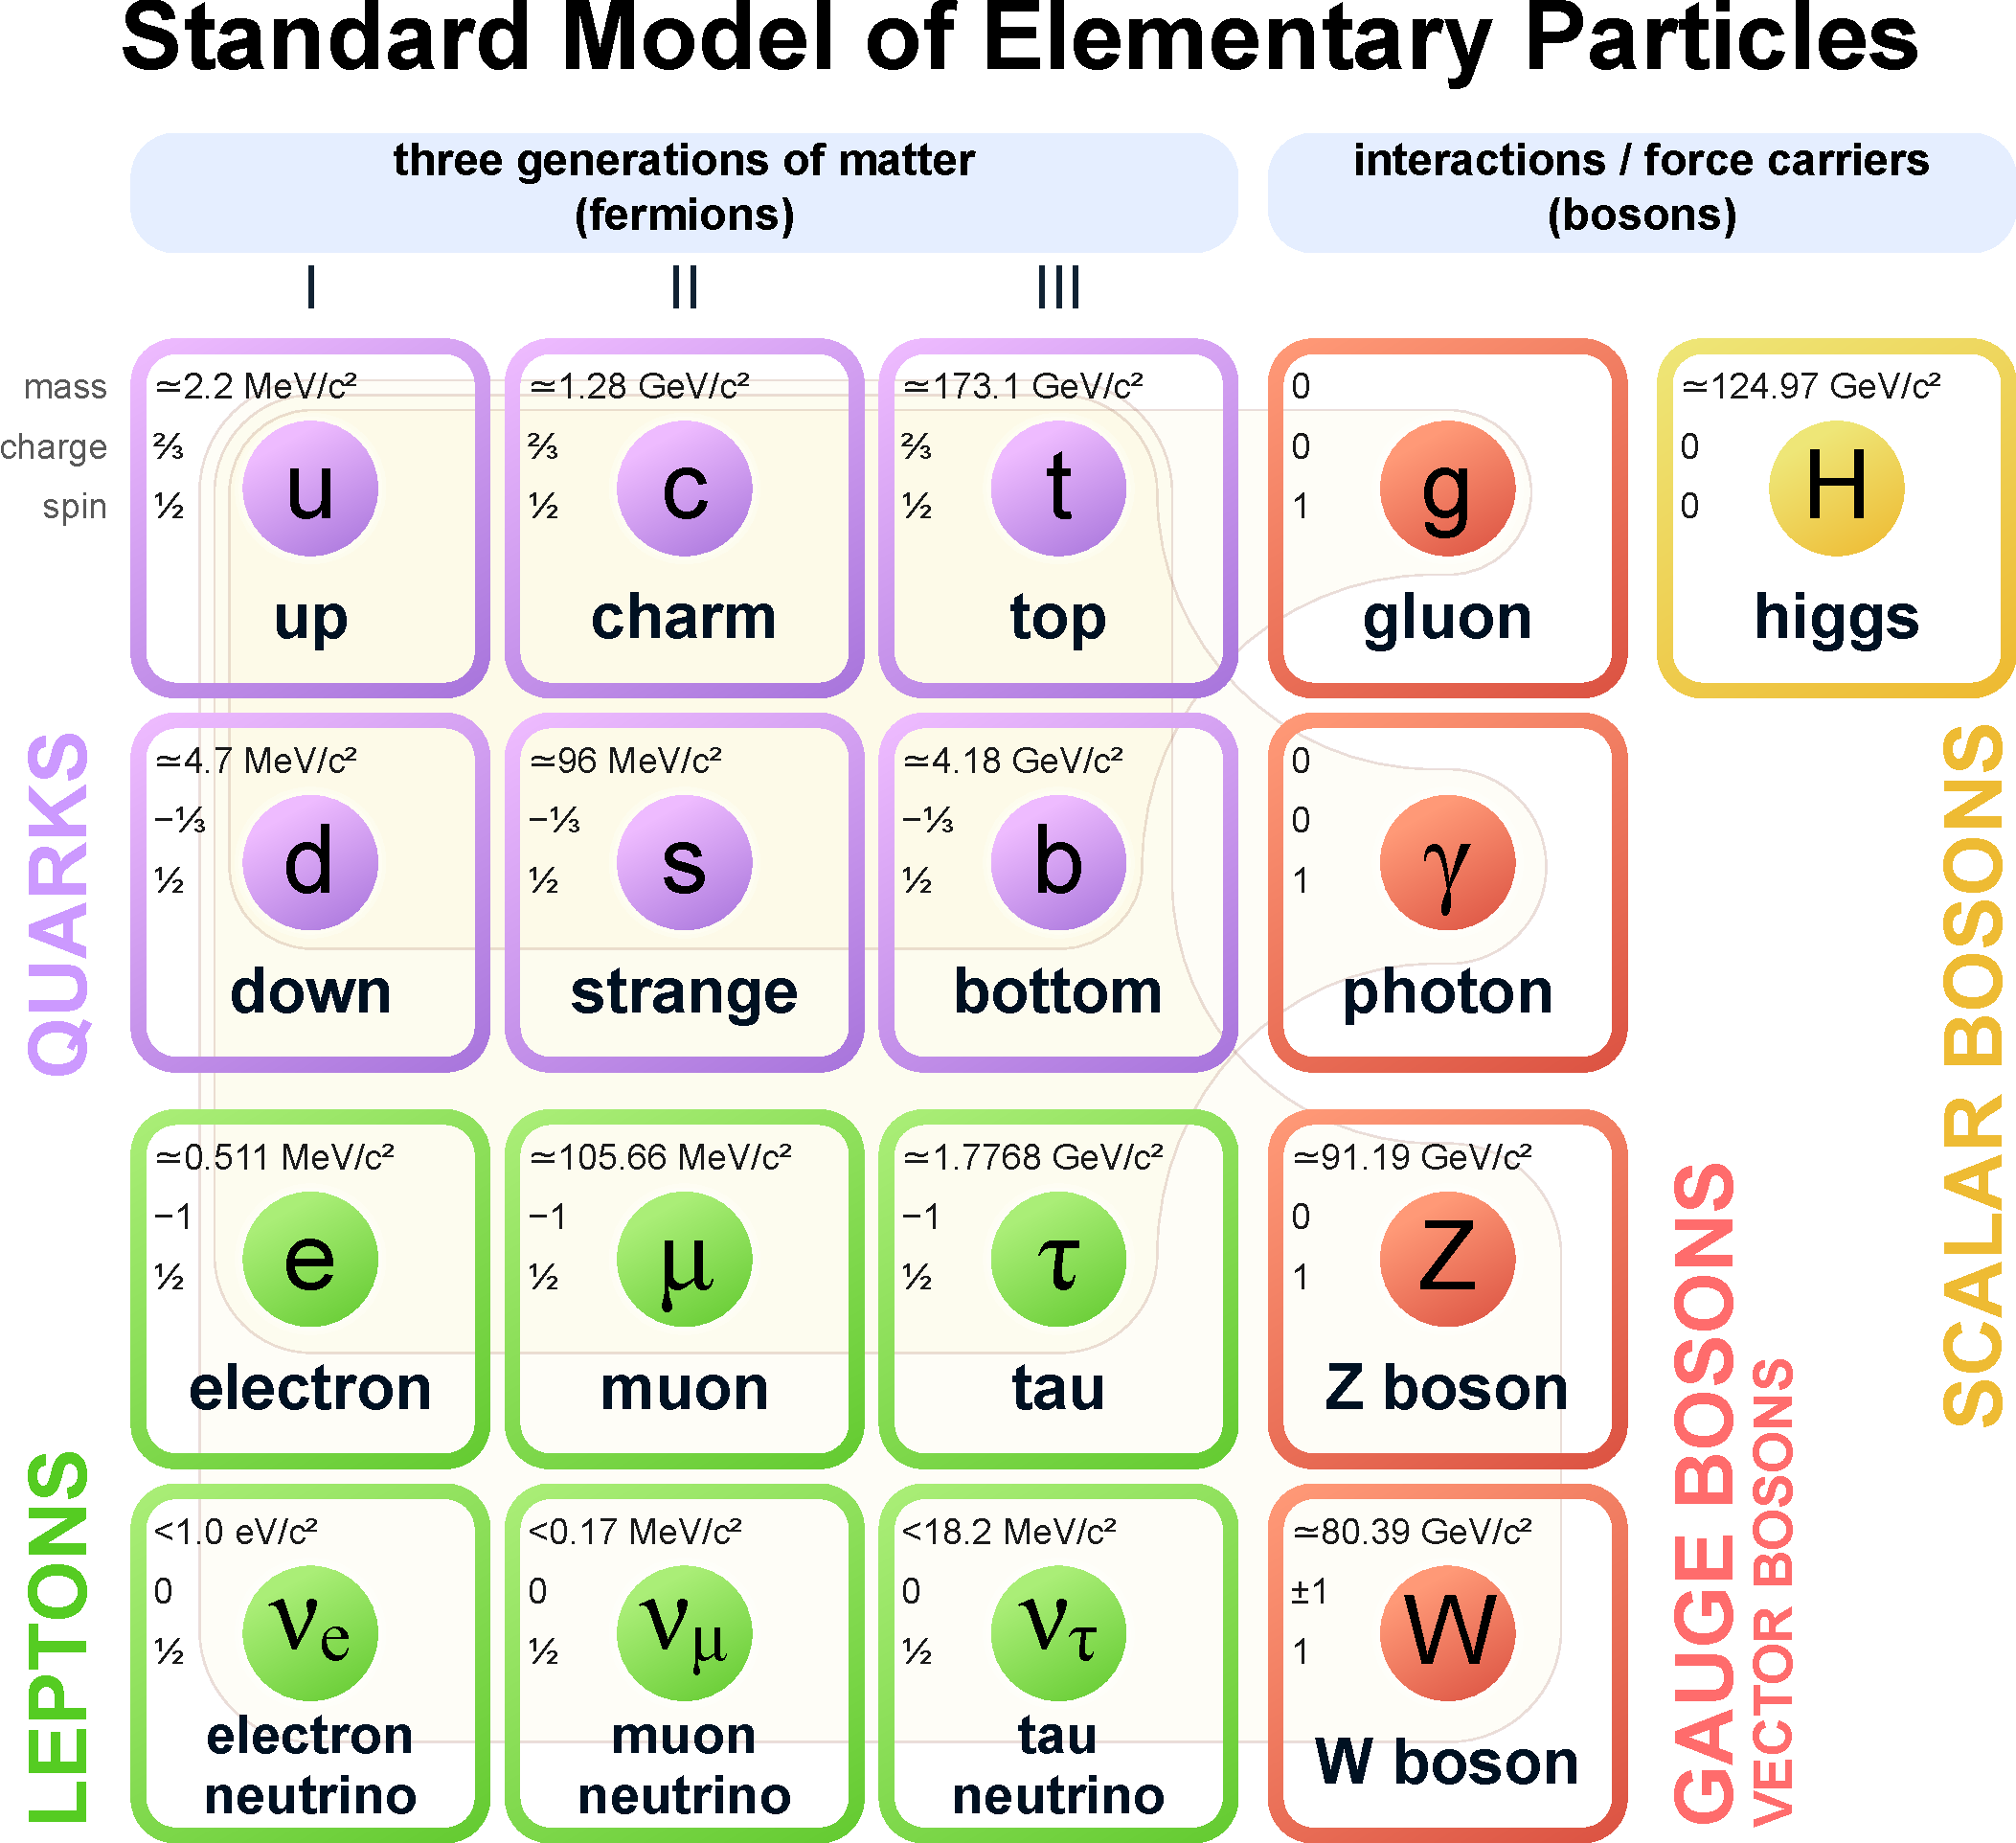
\includegraphics[width=0.6\textwidth]{chap1/Standard_Model_of_Elementary_Particles.pdf}
    \caption{The elementary particles of the Standard Model. Reproduced from
             Wikimedia~\cite{standard_model_wikimedia}.
            }
    \label{fig:Standard_Model_of_Elementary_Particles}
\end{figure}


\section{Electron scattering}
The Thomas Jefferson National Accelerator Facility (JLab) in Newport News, VA
is home to the Continuous Electron Beam Accelerator Facility (CEBAF).
The CEBAF beam delivers a beam of high energy polarized electrons to four
experimental halls.
Most JLab experiments study the debris produced when the electron beam
hits a fixed nuclear target.
By studying this debris, physicists are able to obtain new insights into
nuclear and nucleon structure, exotic configurations of quarks, and other
features of QCD.
Electron beams such as the CEBAF are powerful tools for studying nuclear
structure
because the processes involved in electron-nucleus scattering experiments are
governed by QED (a theory which is very well understood and calculable to high
degrees of precision).

\begin{figure}[H]
    \centering
    \vspace{1cm}
        \begin{fmffile}{chap1/elastic_scattering}
            \setlength{\unitlength}{1cm}
            \begin{fmfgraph*}(8,5)
                \fmfleft{ie,oe}
                \fmfright{ip,op}

                \fmflabel{$(E_e,\vec{p}_e)$}{ie}
                \fmflabel{$(E'_e,\vec{p'}_e)$}{oe}

                \fmflabel{$(E_p,\vec{p}_p)$}{ip}
                \fmflabel{$(E'_p,\vec{p'}_p)$}{op}

                \fmf{fermion}{ie,v1,oe}
                \fmf{photon,label=$q_\mu=(\nu,,\vec{q})$}{v1,v2}
                \fmf{fermion}{ip,v2,op}
            \end{fmfgraph*}
        \end{fmffile}
    \vspace{1cm}
    \caption{Feynman diagram for elastic $ep$ scattering.}
    \label{fig:feynman_ep}
\end{figure}

Consider a situation in which an electron and proton collide.
The tree-level diagram for this process is shown in Fig~\ref{fig:feynman_ep}.
Let $p_e^\mu=(E_e,\vec{p}_e)$ be the incoming four-momentum of the electron and
${p'}_e^\mu=(E'_e,\vec{p'}_e)$ be its outgoing four-momentum.
Similarly, let $p_p^\mu$ and ${p'}_p^\mu$ be the incoming and outgoing
four-momenta of the proton.
The virtual photon carries a four-momentum
$q^\mu=(\nu,\vec{q})=(E_e-E'_e,\vec{p}_e-\vec{p'}_e)$ between the two
particles.
An important quantity defined for such processes is the four-momentum transfer
squared $Q^2=-q^\mu q_\mu$.
Similarly, $\nu=E_e-E'_e$ is the energy transfer.

\textit{Elastic scattering} is a process in which an electron and proton
collide, and both particles retain their identities.
This process can be seen as a distinct peak at $Q^2=2m_p\nu$ on the bottom axis
labeled ``PROTON'' in Fig~\ref{fig:nuclear_response_function}.
This figure is a schematic representation of the nuclear response
function\footnote{The nuclear response function can be thought of as the
probability for an interaction to occur between an electron and a proton or
nucleus at a given value of $Q^2$ and $\nu$.} as a function of $Q^2$ and $\nu$.

For a fixed value of $Q^2$, higher energy transfers $\nu$ result in first
resonances of the proton and, as the virtual photon probes smaller and
smaller distances, eventually deep inelastic scattering (DIS).
DIS processes are possible because the proton is not a point-like particle
without a substructure, but rather a composite particle composed of quarks.
The DIS region extends to electron-nucleus scattering at larger $\nu$ (see the
middle axis labeled ``NUCLEUS.''
In DIS events, quarks can be knocked out of protons and neutrons to form other
hadrons such as pions and kaons.

At lower values of $\nu$ for fixed $Q^2$, there is a peak labeled
quasi-free scattering, which is another term for \textit{quasielastic
scattering}.
This is a process in which the struck proton retains its identity and holds
onto its constituent quarks.
The process ``looks'' more like elastic scattering involving a free proton than
it does an inelastic process.

\begin{figure}[!h]
    \centering
    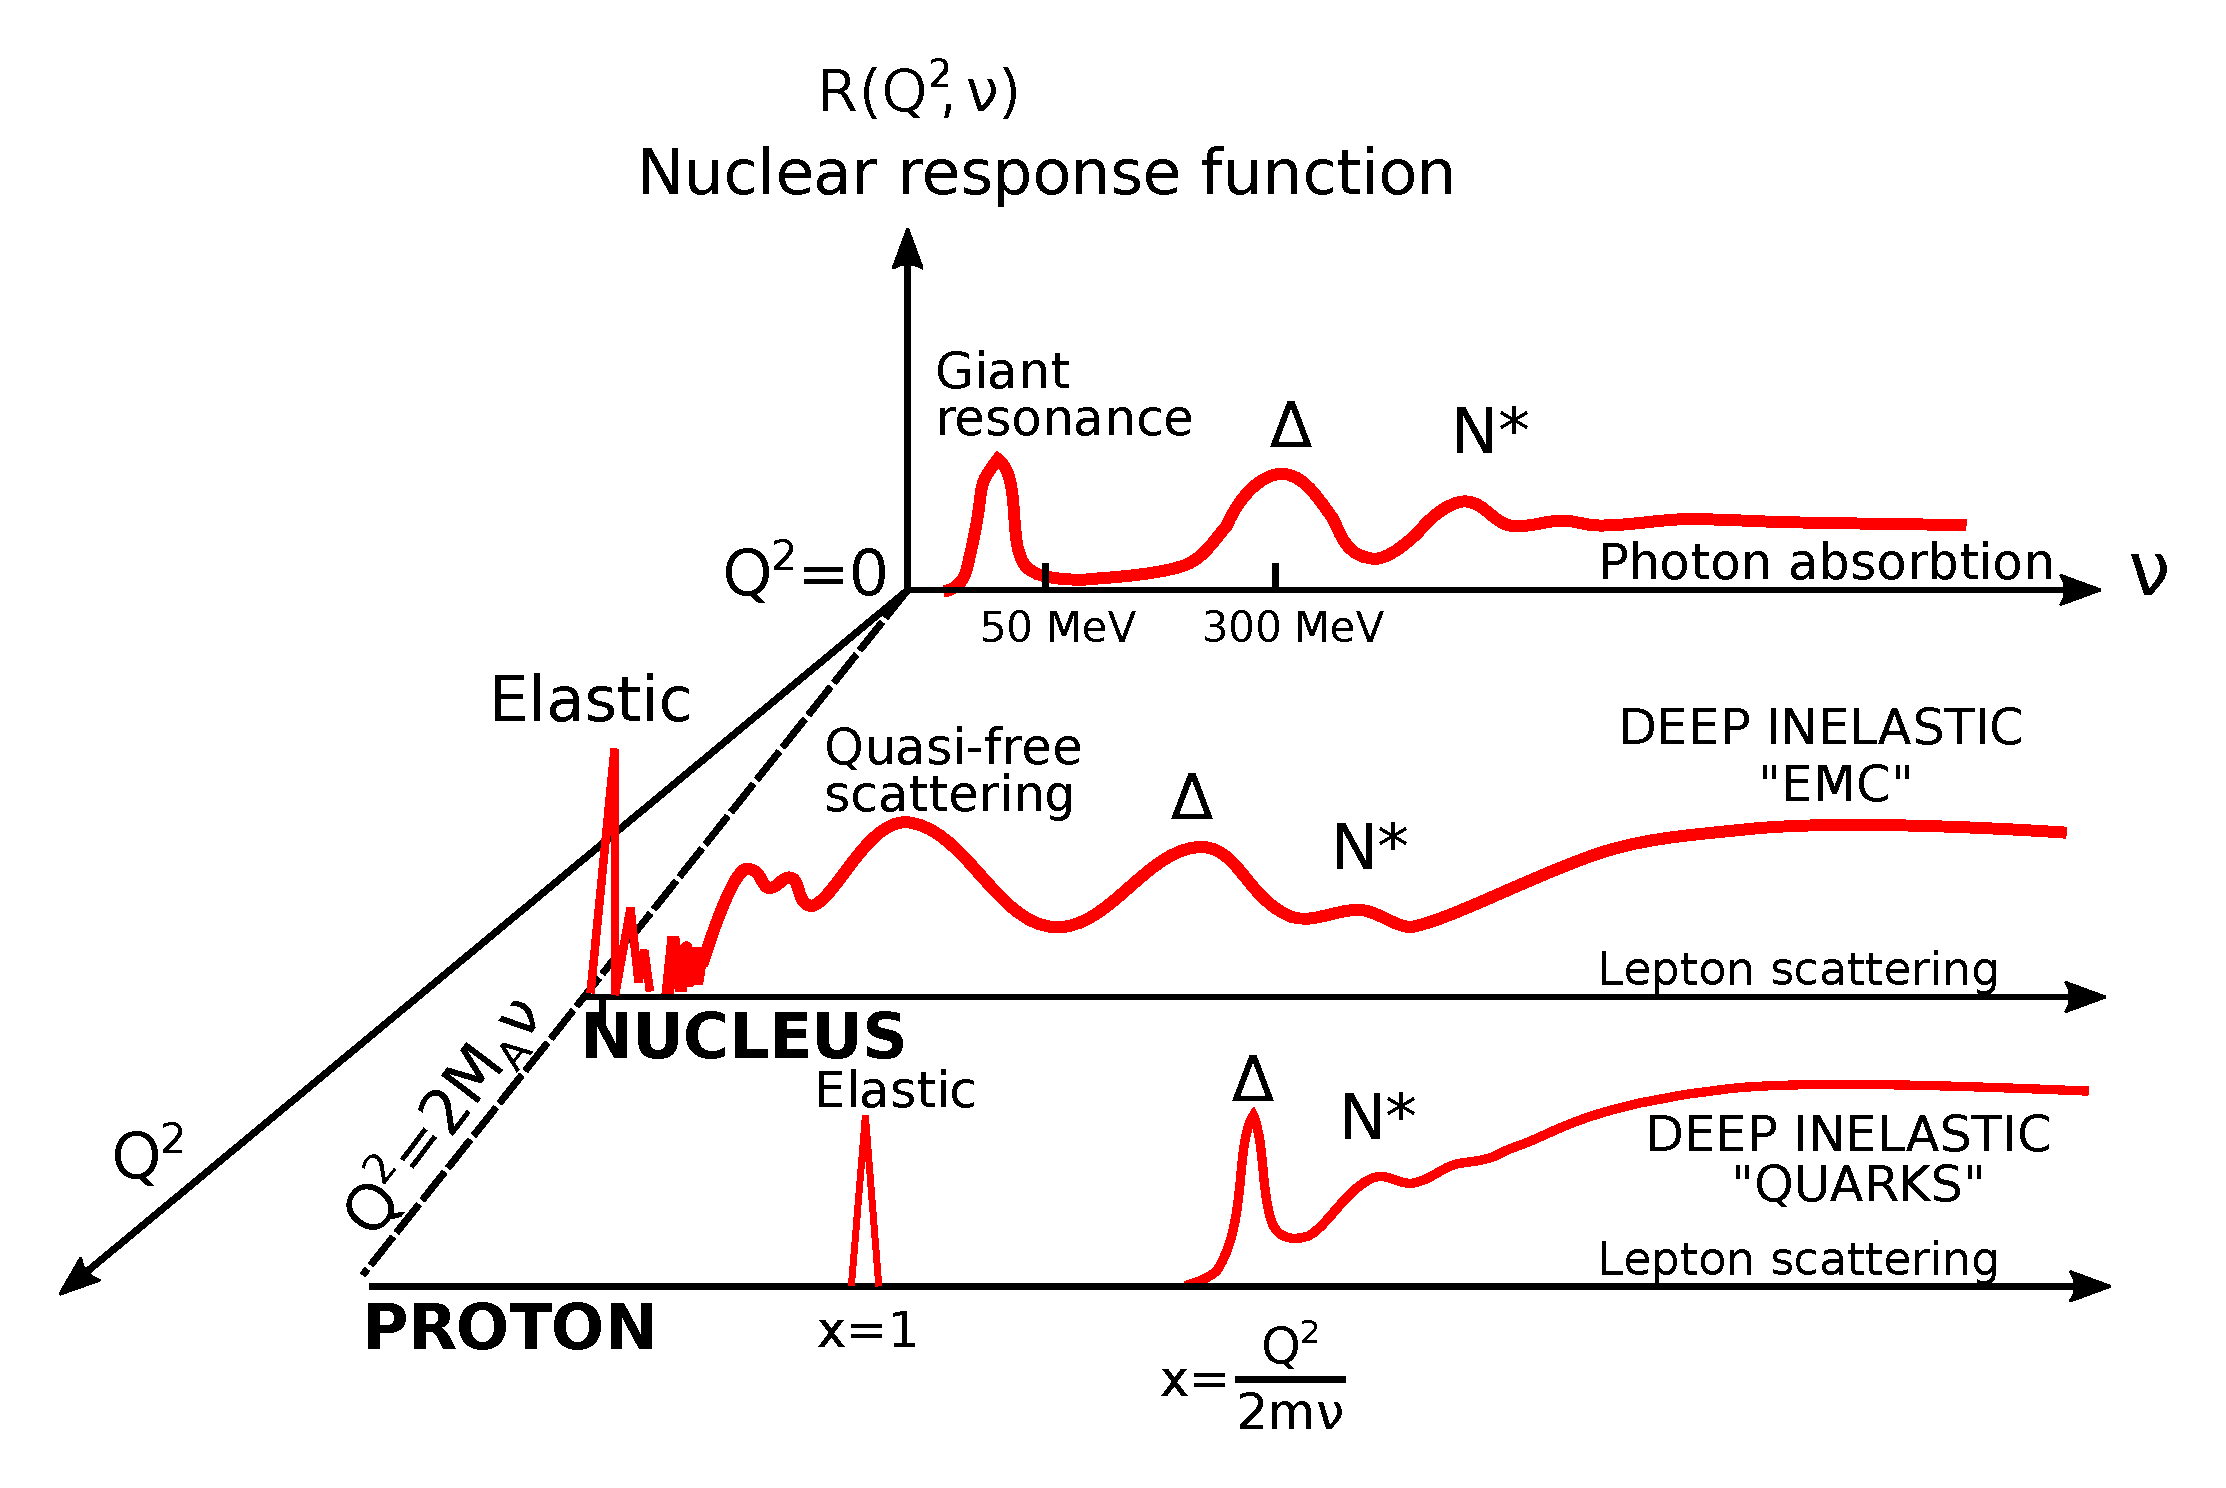
\includegraphics[width=1.0\textwidth]{chap1/nuclear_response_function_new.pdf}
    \caption{
             Reproduced from Ref~\cite{Frois_1985}.
            }
    \label{fig:nuclear_response_function}
\end{figure}

Quasielastic scattering is one type of scattering process that can be studied
in detail at JLab in Hall C using a pair of apparatuses called spectrometers.
If both spectrometers are used in tandem to collect both the scattered electron
and ejected proton, this is called \textit{exclusive} quasielastic scattering.
Inclusive scattering detects only one of the particles, leaving some abmiguity
about exactly what process led to its being scattered into a spectrometer.


Because the ejected proton interacts with the residual nucleons via the strong
force, it will interact with the nuclear medium as it exits the nucleus.
This ``rescattering'' process is well-described by Glauber multiple scattering
theory~\cite{Glauber_1959}.
However, there is a distinctive prediction~\cite{Mueller_1982,Brodsky_1982}
arising from QCD that in exclusive processes at large $Q^2$, initial and final
state interactions (ISI and FSI) such as Glauber multiple scattering vanish.
At sufficienctly large $Q^2$, a proton ejected from a nucleus in quasielastic
scattering behaves as if it were a free proton participating in elastic
scattering.
